\lesson{Hello world}

Die erste Lektion beschäftigt sich alleine mit der Frage, was eigentlich eine
Programmiersprache überhaupt ist und wie wir den Computer dazu bringen können,
daraus etwas zu machen, was er ausführen kann.
Traditionell wird hierfür ein Programm herangezogen, das „Hallo Welt!“ ausgibt. \\


\textbf{Wie entsteht ein Programm?}

Wie bringen wir also den Computer dazu, diese Ausgabe zu generieren? - intern besteht er aus
vielen Transistoren (wenn ihr nicht wisst, was das ist, denkt an winzige
Schalter - näheres folgt im späteren Studium), die nur die Zustände „an“ und „aus“ kennen.
Wir müssen also die Anweisung „gebe Hallo Welt aus“ in ein Format übersetzen, was nur „an“ und
„aus“ bzw. „0“ und „1“ benutzt.

Nun ist es umständlich, ein umfangreiches Programm in 0en und 1en zu schreiben. Deswegen benutzt man
heutzutage so genannte Hochsprachen, um Programme zu beschreiben. Wir
beschreiben also den Programmablauf in einer von Menschen lesbaren und
(leicht) verstehbaren Sprache, welche später in 0en und 1en übersetzt wird und anschließend vom Computer lesbar ist und ausgeführt werden kann.
Wir benutzen die Hochsprache \Cpp. Die Programmbeschreibung in
\Cpp legen wir dabei in einer einfachen Textdatei ab. Damit wir auf anhieb erkennen, um welche Hochsprache es sich handelt, hat es sich etabliert die Endung
\texttt{.cpp} an den Dateinamen anzuhängen.

Die Übersetzung aus der von Menschen lesbarer Hochsprache in Maschinensprache erledigt für uns der \emph{Compiler}.
Der Compiler generiert aus der Textdatei also Maschinencode generiert. Der Compiler für \Cpp, den wir in diesem Kurs
benutzen wollen, heißt \texttt{g++}.

Vereinfacht sieht der Prozess zur Programmerstellung also wie folgt aus:

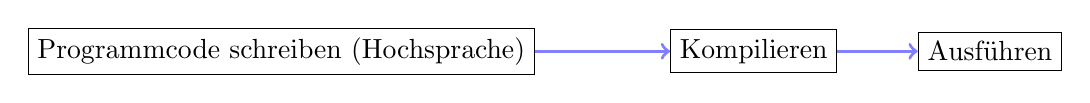
\begin{tikzpicture}
    \node (1) at (0,0) [rectangle, draw] {Programmcode schreiben (Hochsprache)};
    \node (2) at (6,0) [rectangle, draw] {Kompilieren};
    \node (3) at (9,0) [rectangle, draw] {Ausführen};
    \draw[->, blue!50, very thick] (1) to (2);
    \draw[->, blue!50, very thick] (2) to (3);
\end{tikzpicture} \\

\textbf{Wie gehe ich dabei vor?}

Um den Programmcode in eine Textdatei zu schreiben verwenden wir einen Texteditor.
Dies kann mit fast jedem einfachen Texteditor bewerkstelligt werden. Populäre konsolenbasierte Editoren sind \texttt{vim} und \texttt{nano}. Es existieren aber auch grafische Editoren, die speziell für das Schreiben von Programmcode entwickelt wurden, wie \texttt{Visual Studio Code} oder \texttt{CLion}.
Um dem Compiler zusagen, welche Textdatei er in ein Programm übersetzen soll, verwenden wir die sogenannte Shell. Vorerst reicht uns zu wissen, dass die Shell
ein Werkzeug ist, um dem Computer spezifisch zu sagen, was er machen soll (mehr dazu im folgenden Kapitel). In Ubuntu verwenden wir hierzu das Terminal, ebenso in MacOS,
unter Windows CMD oder Powershell. Ein Befehl für \texttt{g++} (dem Compiler für \Cpp) sieht beispielsweise wie folgt aus:

\begin{center}
    \texttt{g++ -o outputDatei zuKompilierendeDatei.cpp}
\end{center}
Hierbei legen wir mit dem Parameter \texttt{-o} (o für output) und dem ersten darauf folgenden Argument den Namen der Ausgabedatei fest.

Nachdem \texttt{g++} uns also ein Maschinencodefile -- die \texttt{outputDatei} --
erzeugt hat, können wir es zur Ausführung bringen. Dies kann im Terminal mit einem Punkt und einem Slash vor dem Dateinamen geschehen. Also:
\begin{center}
    \texttt{./outputDatei}
\end{center}



\begin{praxis}

    \textbf{Erstes Programm in \Cpp schreiben}

    \begin{enumerate}
        \item Erstelle eine neue, leere Datei in einem Editor deiner Wahl.
        
        \item Kopiere folgenden Programmcode in den Texteditor und speichere ihn in einer Datei mit dem Namen „helloworld.cpp“ ab. 
        Das nähere Verständnis des Programmcodes ist an dieser Stelle nicht notwendig. 
    \end{enumerate}    

    \inputcpp{helloworld.cpp}

    \textbf{\Cpp-Code komplieren und Programm erstellen }
  
    \begin{enumerate}
        \item Öffne ein Terminal (Konsole), ihr findet das Terminal unter Ubuntu oben links unter „Applications“ als „Terminal“ oder mittig unten als das zweite Symbol von links.
        \item Wechselt mit dem Befehl \texttt{cd [PFAD]} in das Verzeichnis (Ordner), indem ihr eure Textdatei erstellt habt (\texttt{[PFAD]} muss hierbei durch den Speicherort der Datei ersetzt werden).
              Was dieser Befehl genau tut und wie er funktioniert, erfahrt ihr in Lektion 2.
        \item In diesem Verzeichnis liegt nun eine Datei mit dem Namen \texttt{helloworld.cpp}.
              Benutzt \texttt{g++}, um diese zu einer Datei (in diesem Fall dem Programm) \texttt{hello} zu
              kompilieren. Orientiert euch dazu an den folgenden Befehlen. (siehe Diagramm)
        \item Führt die Datei \texttt{hello} aus.
    \end{enumerate}
\end{praxis}


Zur besseren Übersichtlichkeit hier der ganze Vorgang noch mal in einem
Diagramm:

% TODO: Buttugly, but well... - its gonna stay this way
\begin{center}
    \resizebox{\textwidth}{!}{
        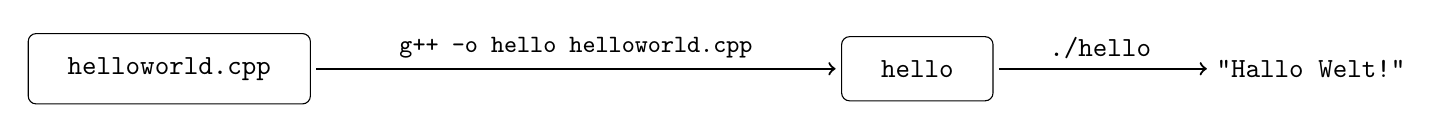
\begin{tikzpicture}
            \node (nHelloWorldCpp) [ shape=rectangle, rounded corners = 0.1cm, draw=black, inner xsep=0.5cm, inner ysep = 0.3cm ] {\texttt{helloworld.cpp}};
            \node (nHello) [ right of = nHelloWorldCpp, node distance = 9.5cm, shape=rectangle, rounded corners = 0.1cm, draw = black, inner xsep = 0.5cm, inner ysep = 0.3cm ] {\texttt{hello}};
            \draw [->, thick, shorten >= 2pt, shorten <= 2pt ] (nHelloWorldCpp) -- (nHello) node [ midway, above, font = \small ] { \texttt{g++ -o hello helloworld.cpp}} ;
            \node (nOutput) [ right of = nHello, node distance = 5cm, shape=rectangle ] {\texttt{"Hallo Welt!"}};
            \draw [->, thick, shorten <= 2pt] (nHello) -- (nOutput) node [ midway, above ] {\texttt{./hello}};
        \end{tikzpicture}
    }
\end{center}

\newpage

\begin{spiel}

Ihr könnt nun versuchen, den Quellcode selbst zu verändern und damit ein wenig
herumzuspielen. Öffnet dazu einen Editor und öffnet die Datei
\texttt{vorkurs/lektion01/helloworld.cpp}\footnote{am besten öffnet ihr in VSCode den gesamten Vorkurs-Ordner}. Denkt daran, nach jeder Änderung die Datei zu speichern und
im Terminal neu zu kompilieren und auszuführen.

Dinge, die ihr ausprobieren könntet sind zum Beispiel:
\begin{enumerate}
    \item Was passiert, wenn ihr „Hello world!“ in etwas anderes ändert?
    \item Was passiert, wenn ihr die erste Zeile löscht (der Originalquellcode
        ist in diesem pdf enthalten, ihr könnt sie also später wieder
        herstellen)?
    \item Was passiert, wenn ihr das „\verb|<< std::endl|“ löscht?
    \item Wie könnte man mehrere Sätze ausgeben? Wie könnte man mehrere Zeilen
        ausgeben?
\end{enumerate}
\end{spiel}

\textbf{Quiz 1}\\
\textit{Was passiert, wenn ihr \texttt{Hello world} durch etwas anderes ersetzt?}
\begin{enumerate}[label=\alph*)]
    \item Das andere wird ausgegeben
    \item Es gibt einen Fehler
    \item Das Programm tut garnichts mehr
    \item Das Programm gibt trotzdem \texttt{Hello world} aus
\end{enumerate}